% This file was created by matplotlib2tikz v0.7.4.
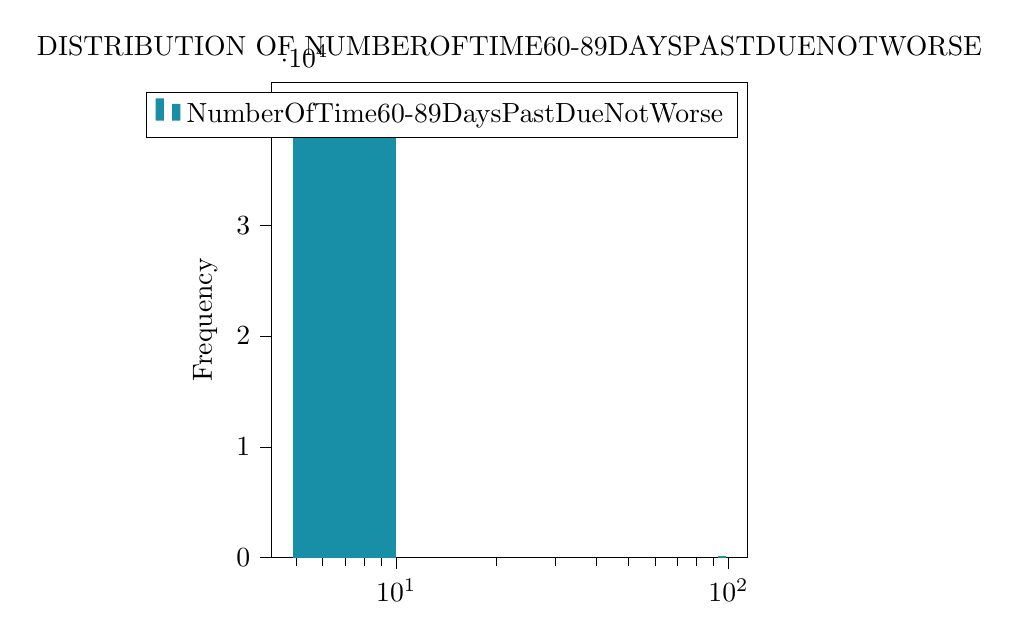
\begin{tikzpicture}

\definecolor{color0}{rgb}{0.0941176470588235,0.56078431372549,0.654901960784314}

\begin{axis}[
height=3in,
log basis x={10},
tick align=outside,
tick pos=left,
title={\printsubsection{\MakeUppercase{Distribution of NumberOfTime60-89DaysPastDueNotWorse}}\\},
width=3in,
x grid style={white!69.01960784313725!black},
xmin=4.2183691307255, xmax=113.835462264871,
xmode=log,
xtick style={color=black},
y grid style={white!69.01960784313725!black},
ylabel={Frequency},
ymin=0, ymax=42913.5,
ytick style={color=black}
]
\draw[fill=color0,draw opacity=0] (axis cs:0,0) rectangle (axis cs:4.9,40870);
\addlegendimage{ybar,ybar legend,fill=color0,draw opacity=0};
\addlegendentry{NumberOfTime60-89DaysPastDueNotWorse}

\draw[fill=color0,draw opacity=0] (axis cs:4.9,0) rectangle (axis cs:9.8,31);
\draw[fill=color0,draw opacity=0] (axis cs:9.8,0) rectangle (axis cs:14.7,1);
\draw[fill=color0,draw opacity=0] (axis cs:14.7,0) rectangle (axis cs:19.6,0);
\draw[fill=color0,draw opacity=0] (axis cs:19.6,0) rectangle (axis cs:24.5,0);
\draw[fill=color0,draw opacity=0] (axis cs:24.5,0) rectangle (axis cs:29.4,0);
\draw[fill=color0,draw opacity=0] (axis cs:29.4,0) rectangle (axis cs:34.3,0);
\draw[fill=color0,draw opacity=0] (axis cs:34.3,0) rectangle (axis cs:39.2,0);
\draw[fill=color0,draw opacity=0] (axis cs:39.2,0) rectangle (axis cs:44.1,0);
\draw[fill=color0,draw opacity=0] (axis cs:44.1,0) rectangle (axis cs:49,0);
\draw[fill=color0,draw opacity=0] (axis cs:49,0) rectangle (axis cs:53.9,0);
\draw[fill=color0,draw opacity=0] (axis cs:53.9,0) rectangle (axis cs:58.8,0);
\draw[fill=color0,draw opacity=0] (axis cs:58.8,0) rectangle (axis cs:63.7,0);
\draw[fill=color0,draw opacity=0] (axis cs:63.7,0) rectangle (axis cs:68.6,0);
\draw[fill=color0,draw opacity=0] (axis cs:68.6,0) rectangle (axis cs:73.5,0);
\draw[fill=color0,draw opacity=0] (axis cs:73.5,0) rectangle (axis cs:78.4,0);
\draw[fill=color0,draw opacity=0] (axis cs:78.4,0) rectangle (axis cs:83.3,0);
\draw[fill=color0,draw opacity=0] (axis cs:83.3,0) rectangle (axis cs:88.2,0);
\draw[fill=color0,draw opacity=0] (axis cs:88.2,0) rectangle (axis cs:93.1,0);
\draw[fill=color0,draw opacity=0] (axis cs:93.1,0) rectangle (axis cs:98,114);
\end{axis}

\end{tikzpicture}